\section{Presenza di ostacoli}
Gli ambienti visti fino ad ora non presentano alcun tipo di ostacolo, quindi un nodo è vincolato nel movimento solo dalla presenza nelle sue vicinanze di eventuali altri suoi simili. \newline
Per descrivere in maniera più dettagliata uno scenario, è necessario considerare anche la presenza di oggetti al suo interno, che in relazione alla loro grandezza e alla loro posizione possono incidere significativamente sui tempi necessari ad un pedone per scappare o raggiungere una determinata zona.

\subsection{Descrizione della simulazione}
Grazie all'uso dell'\texttt{ImageEnvironment} è stato possibile definire un ambiente contenente cinque ostacoli: quattro rettangolari rispettivamente in alto, in basso, a destra e a sinistra della scena ed uno circolare al centro di essa. \newline
Si è pensato di collocare tre insiemi di pedoni nelle vicinanze di questi oggetti e di definire una zona di sicurezza comune, avendo cura che vi fosse almeno un elemento di intralcio tra essa ed un qualsiasi agente. \newline
La simulazione è stata eseguita prima non considerando il comportamento di steering dell'aggiramento degli ostacoli, poi inserendolo tra le azioni.

\subsection{Risultati ottenuti}
Mentre nella prima simulazione molti nodi rimangono attaccati agli ostacoli, nel vano tentativo di volerci passare attraverso per raggiungere la zona di loro interesse (figura \ref{fig:no-obstacle-avoidance}), nella seconda tutti i pedoni riescono ad arrivare a destinazione, schivando i vari oggetti nella direzione loro più congeniale in relazione alla posizione da cui erano partiti. Il tragitto percorso è deducibile dalla figura \ref{fig:obstacle-avoidance}.

\begin{figure}
    \centering
    \begin{subfigure}[b]{0.75\textwidth}
        \centering
        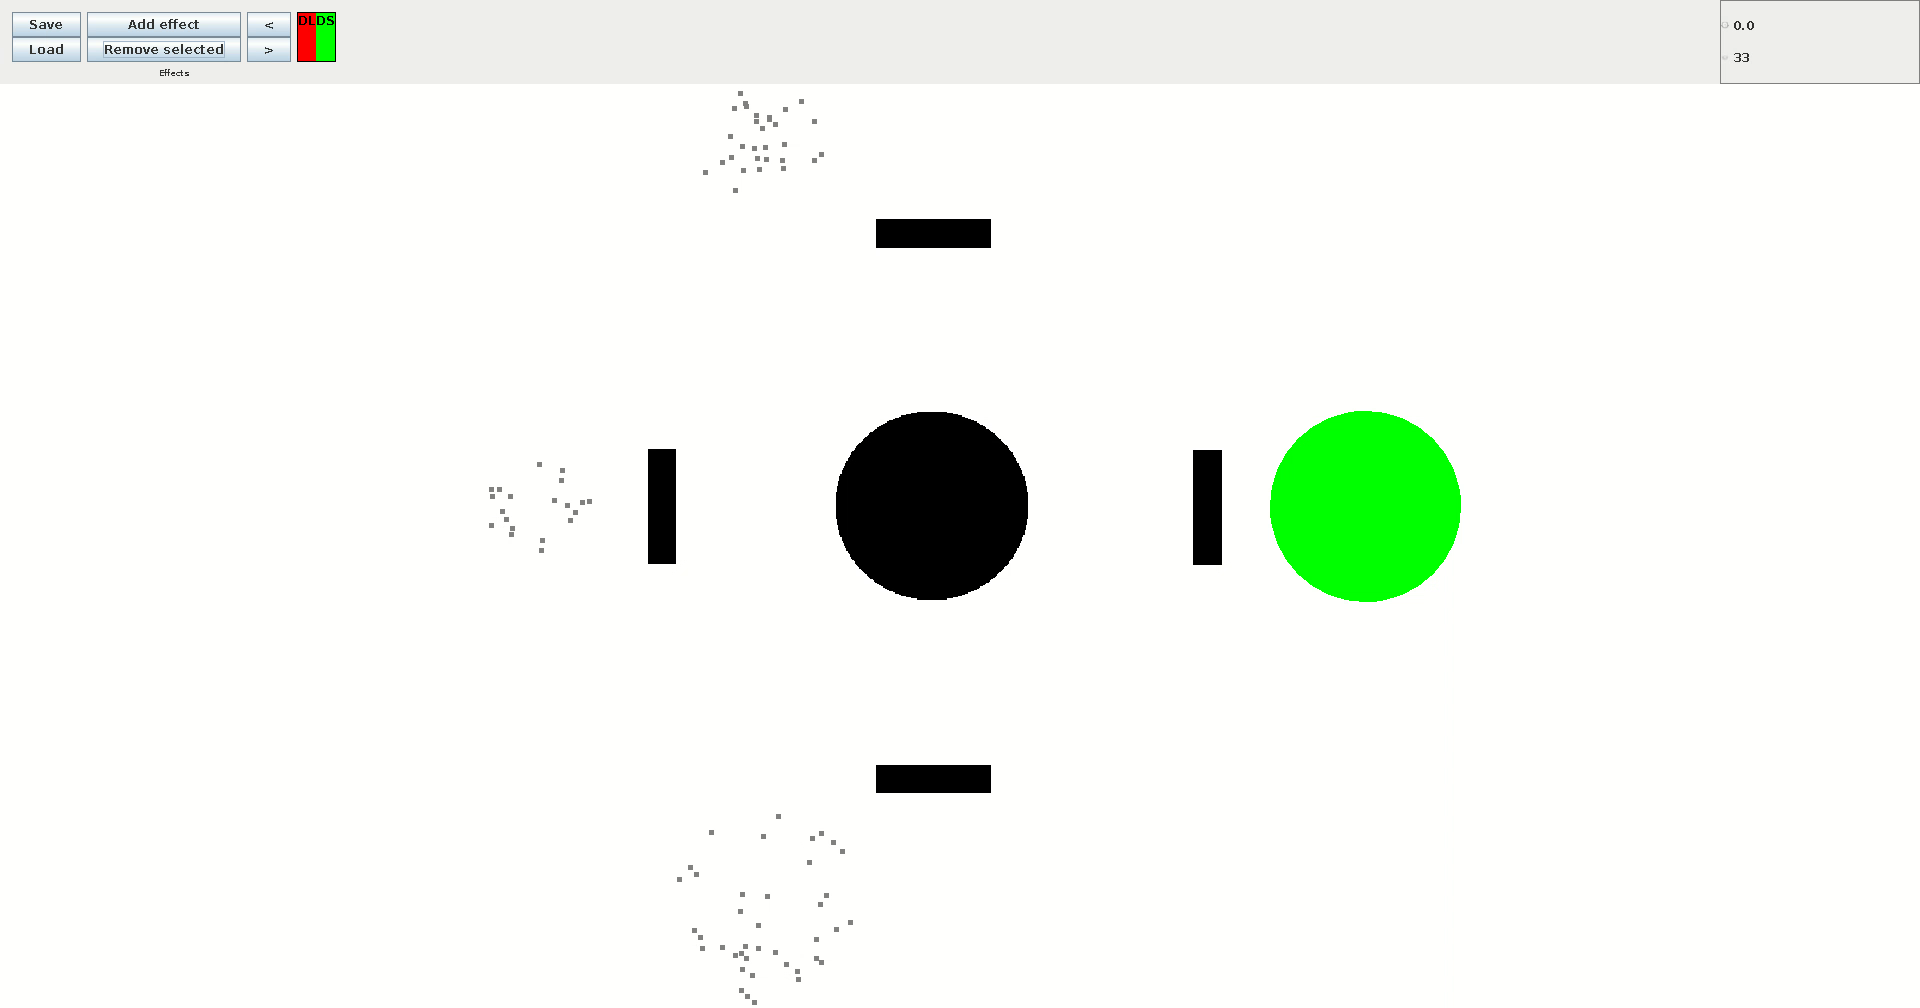
\includegraphics[width=\textwidth]{immagini/casi-studio/no-obstacle-avoidance-begin.png}
    \end{subfigure}
    \hfill
    \begin{subfigure}[b]{0.75\textwidth}
        \centering
        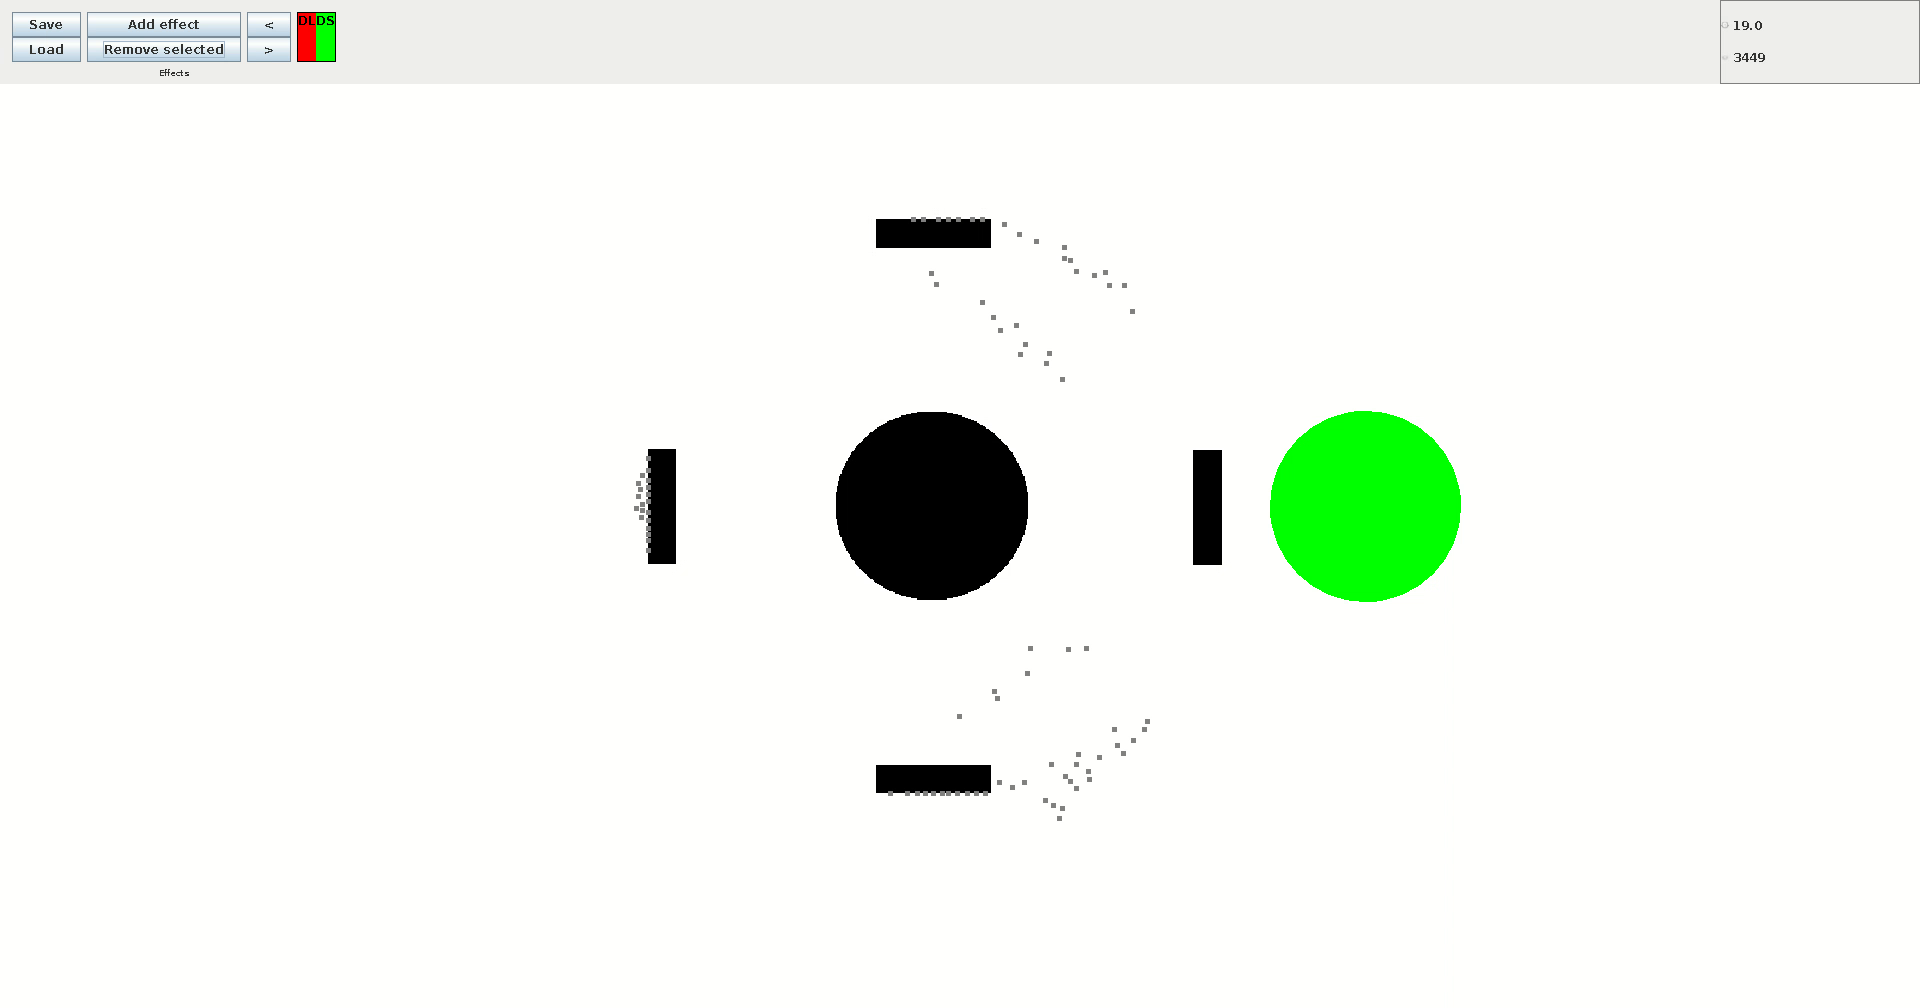
\includegraphics[width=\textwidth]{immagini/casi-studio/no-obstacle-avoidance-during.png}
    \end{subfigure}
    \hfill
    \begin{subfigure}[b]{0.75\textwidth}
        \centering
        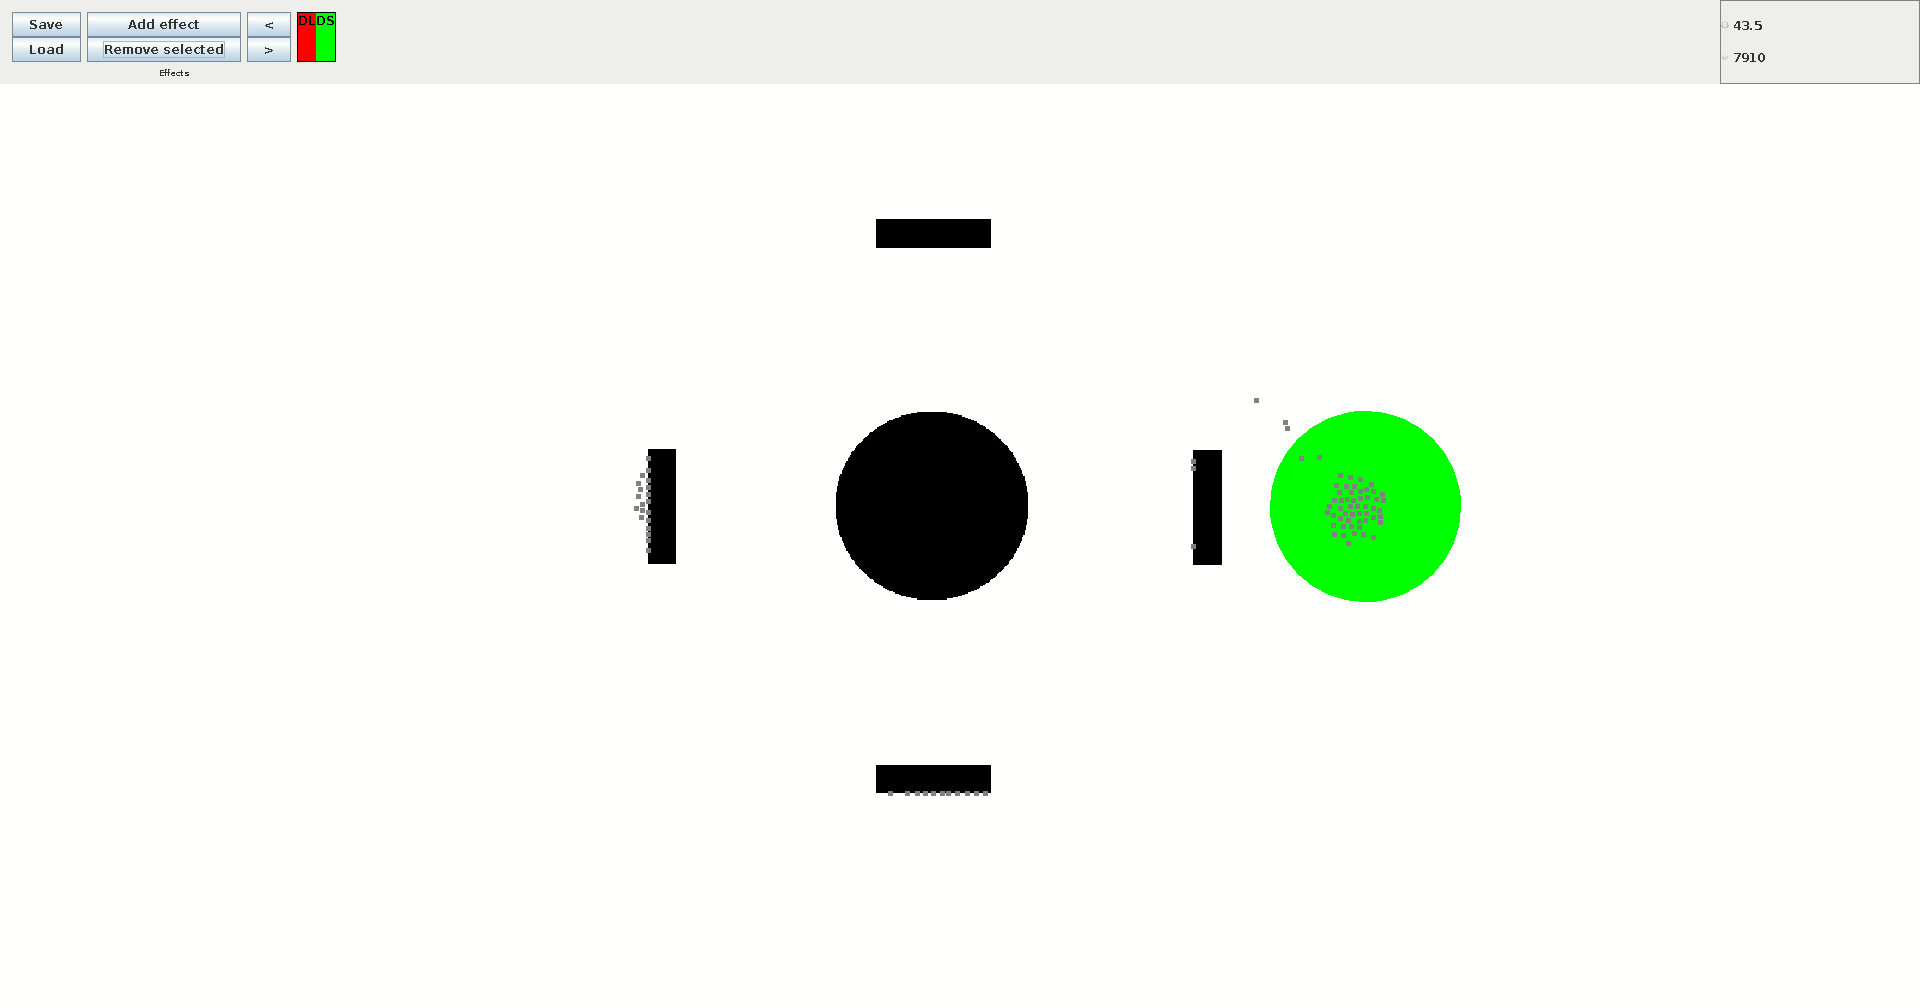
\includegraphics[width=\textwidth]{immagini/casi-studio/no-obstacle-avoidance-end.png}
    \end{subfigure}
    \caption{Fotogrammi salienti della simulazione in cui sono presenti ostacoli non considerando il comportamento di steering ad essi associato; molti pedoni rimangono bloccati durante il loro percorso e non riescono a raggiungere la zona di sicurezza.}
    \label{fig:no-obstacle-avoidance}
\end{figure}

\begin{figure}
    \centering
    \begin{subfigure}[b]{0.75\textwidth}
        \centering
        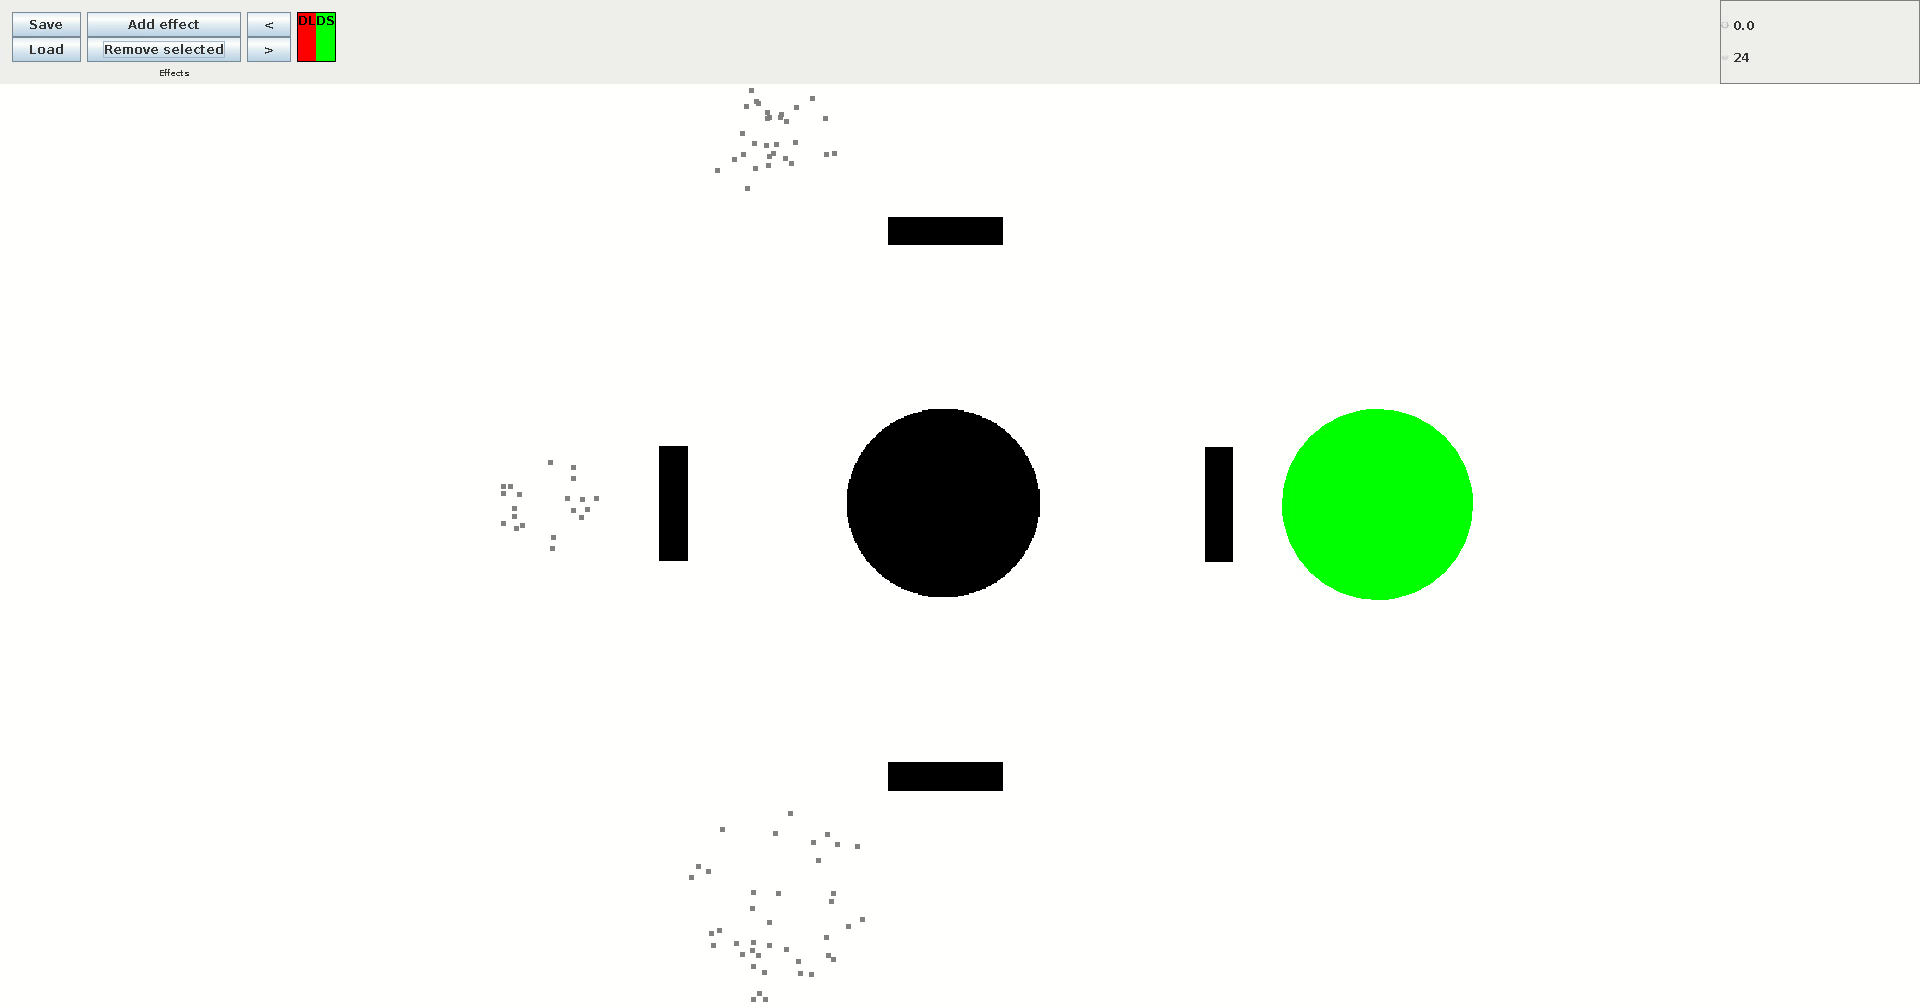
\includegraphics[width=\textwidth]{immagini/casi-studio/obstacle-avoidance-begin.png}
    \end{subfigure}
    \hfill
    \begin{subfigure}[b]{0.75\textwidth}
        \centering
        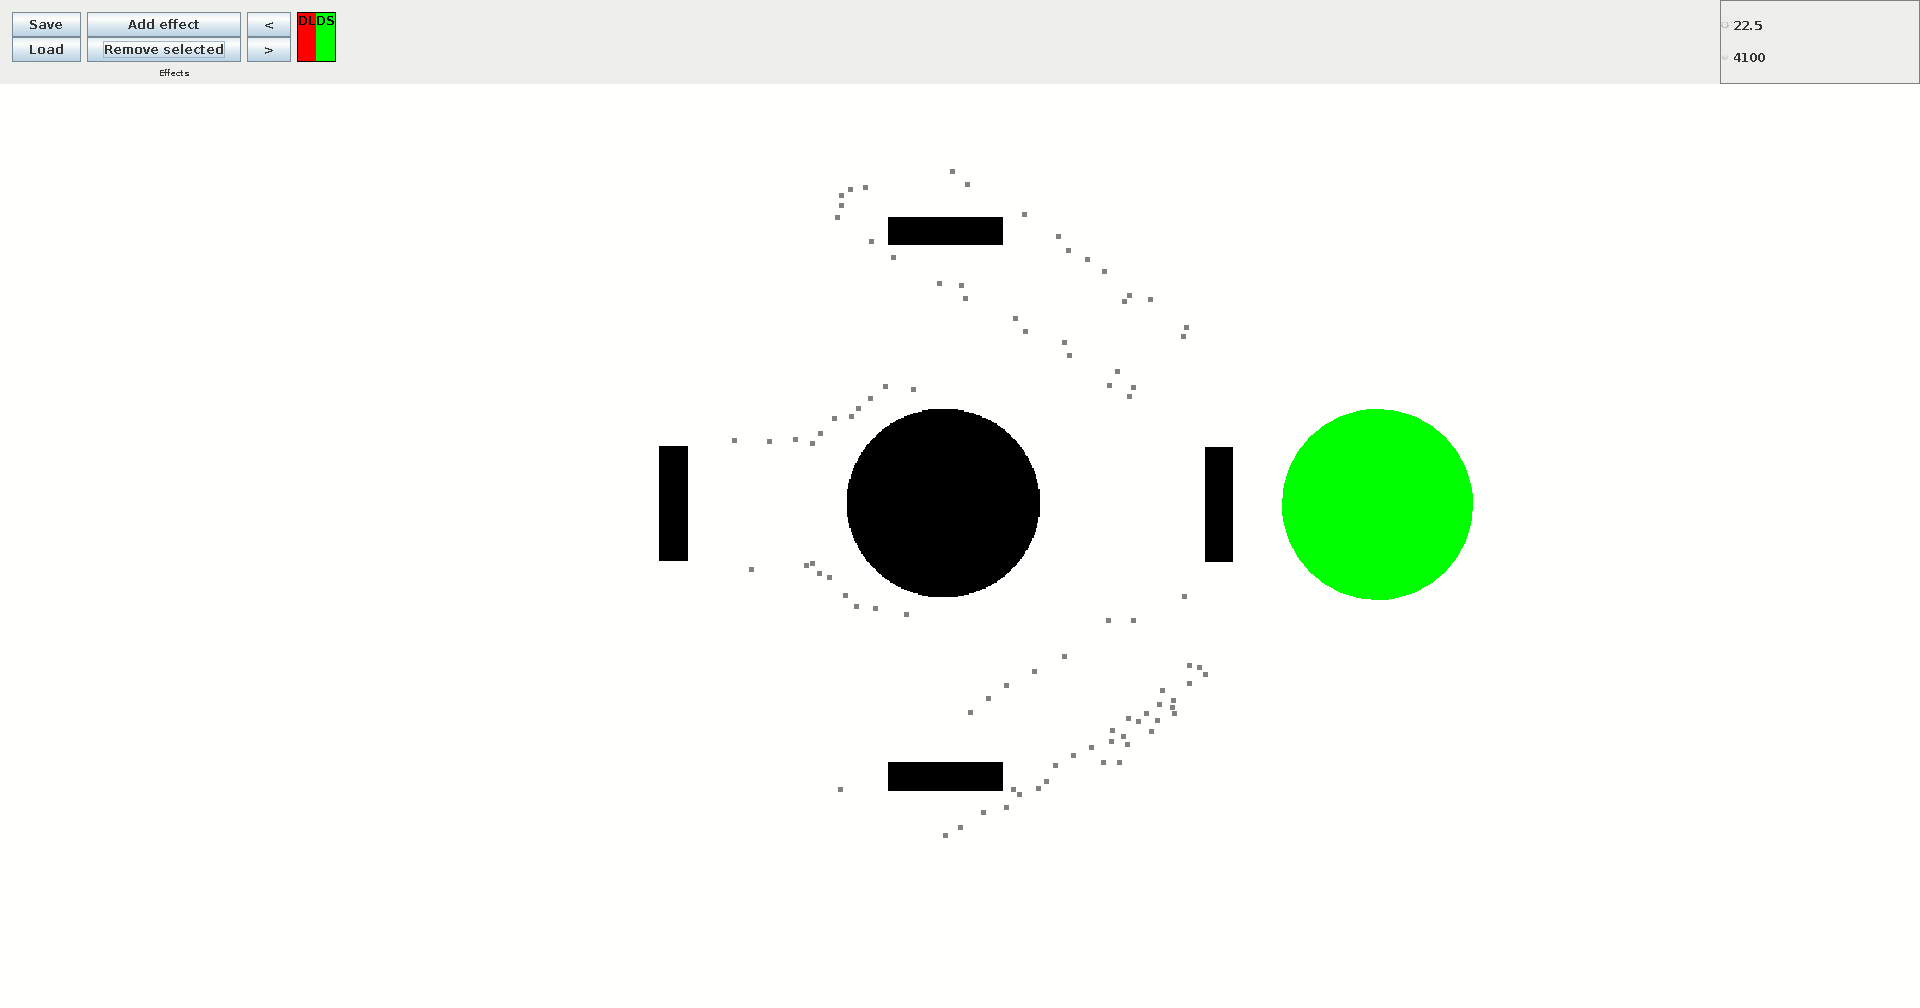
\includegraphics[width=\textwidth]{immagini/casi-studio/obstacle-avoidance-during.png}
    \end{subfigure}
    \hfill
    \begin{subfigure}[b]{0.75\textwidth}
        \centering
        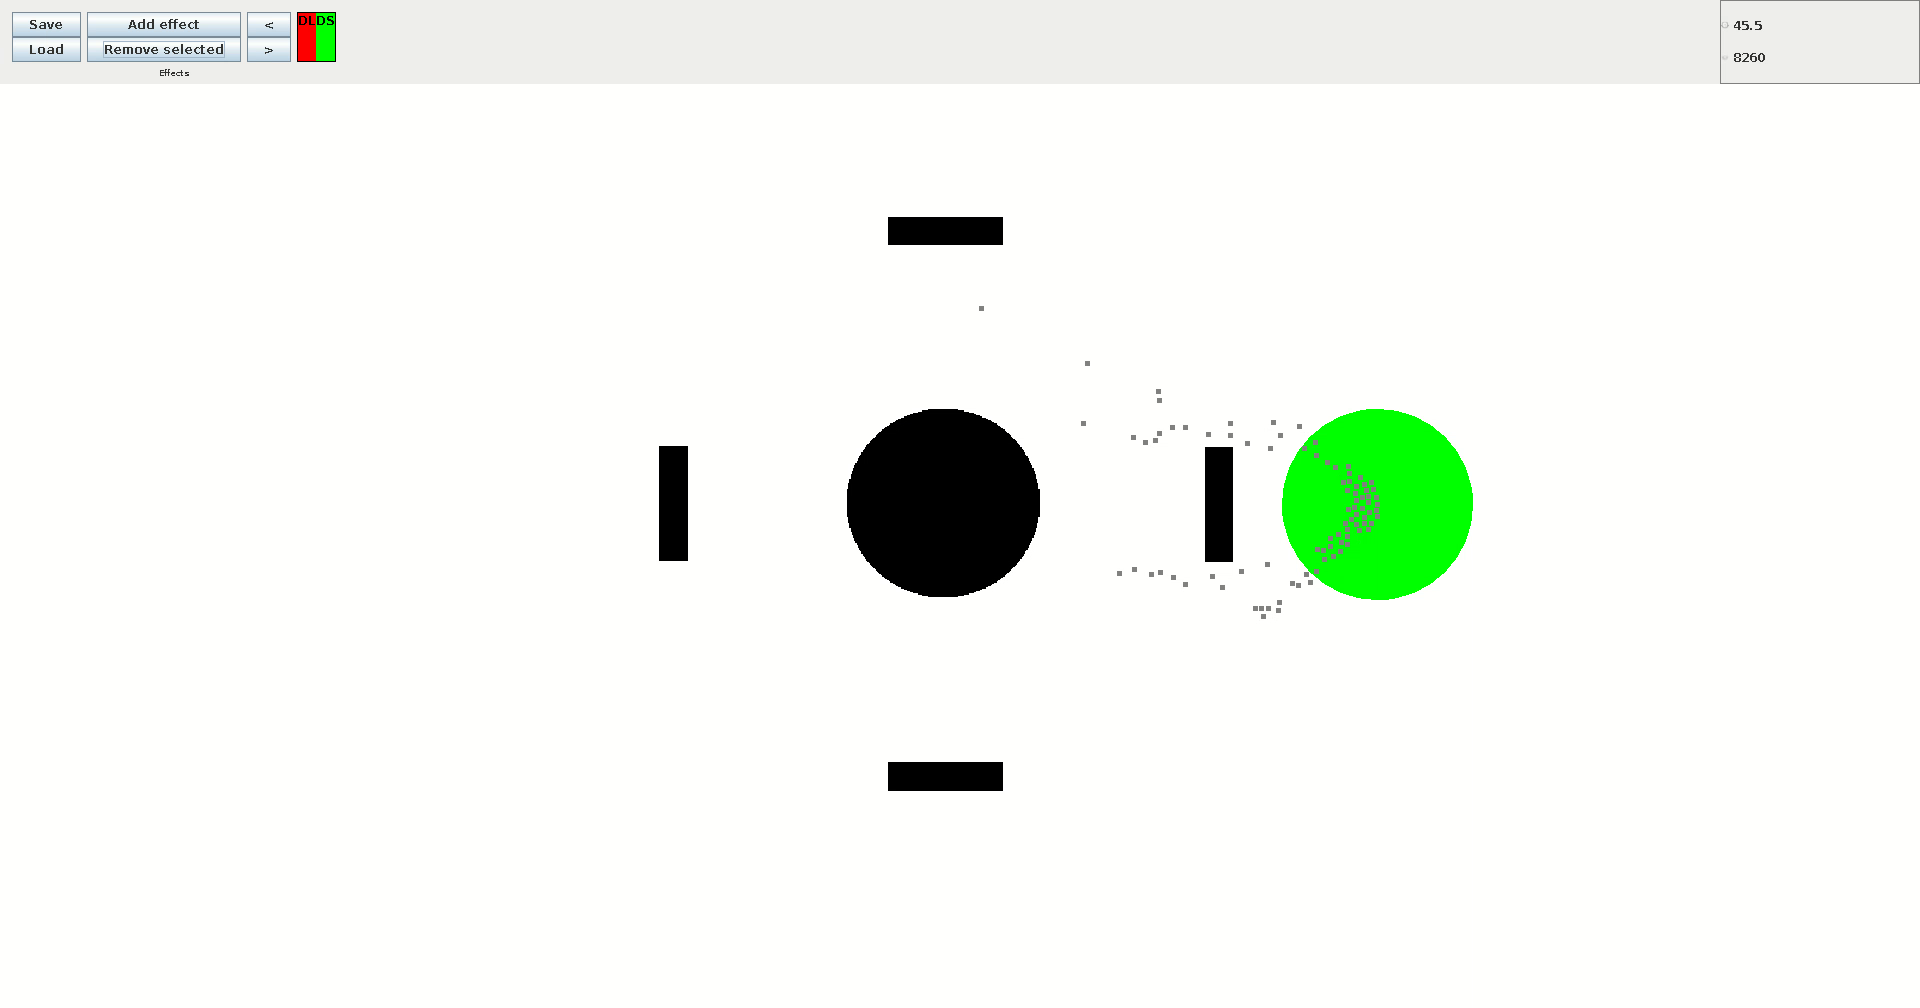
\includegraphics[width=\textwidth]{immagini/casi-studio/obstacle-avoidance-end.png}
    \end{subfigure}
    \caption{Fotogrammi salienti della simulazione in cui sono presenti ostacoli considerando il comportamento di steering ad essi associato; tutti i pedoni riescono a raggiungere la zona di sicurezza evitando eventuali oggetti presenti sul loro cammino.}
    \label{fig:obstacle-avoidance}
\end{figure}